\documentclass[conference]{IEEEtran}
\IEEEoverridecommandlockouts
% The preceding line is only needed to identify funding in the first footnote. If that is unneeded, please comment it out.
\usepackage{cite}
\usepackage{amsmath,amssymb,amsfonts}
\usepackage{algorithmic}
\usepackage{graphicx}
\usepackage{textcomp}
\usepackage[utf8]{inputenc}
\usepackage{listings}
\lstset{language=bash,
  numberstyle=\footnotesize,
  basicstyle=\ttfamily\footnotesize,
  numbers=left,
  stepnumber=1,
  frame=shadowbox,
  breaklines=true}
\usepackage{color}
\usepackage{tabularx,ragged2e,booktabs,caption}
\newcolumntype{C}[1]{>{\Centering}m{#1}}
\renewcommand\tabularxcolumn[1]{C{#1}}
\usepackage[most]{tcolorbox}
% \newtcblisting{commandshell}{colback=white,colupper=gray,colframe=gray!75!black,
% listing only,listing options={language=sh},
% every listing line={\textcolor{black}{\small\ttfamily\bfseries \$> }}}

\usepackage[english,ngerman,brazilian]{babel}
% \begin{filecontents*}{references.bib}
% * <fredguth@fredguth.com> 2018-03-25T07:25:44.547Z:
%
% ^.
% @article{Khoe:1994:CML:2288694.2294265,
%     author = {Khoe, G. -D.},
%     title = {Coherent multicarrier lightwave technology for flexible capacity networks},
%     journal = {Comm. Mag.},
%     issue_date = {March 1994},
%     volume = {32},
%     number = {3},
%     month = mar,
%     year = {1994},
%     issn = {0163-6804},
%     pages = {22--33},
%     numpages = {12},
%     url = {http://dx.doi.org/10.1109/35.267438},
%     doi = {10.1109/35.267438},
%     acmid = {2294265},
%     publisher = {IEEE Press},
%     address = {Piscataway, NJ, USA},
% }
% \end{filecontents*}
\def\BibTeX{{\rm B\kern-.05em{\sc i\kern-.025em b}\kern-.08em
    T\kern-.1667em\lower.7ex\hbox{E}\kern-.125emX}}
    
\begin{document}

\title{Projeto 01 - Explorando OpenCV}

\author{\IEEEauthorblockN{Frederico Guth}
\IEEEauthorblockA{\textit{Aluno Especial, Tópicos em Sistemas de Computação (316491),} \\
\textit{Turma TC - Visão Computacional (PPGI)}\\
\textit{UNB}\\
Brasília, Brasil\\
fredguth@fredguth.com}
}

\maketitle

\section{Objetivos}
Este projeto tem como objetivo principal a exploração e desenvolvimento de algoritmos na ferramenta OpenCV\cite{opencv_library}. 
\section{Introdução}
OpenCV é uma importante biblioteca de código-aberto de rotinas para Visão Computacional\cite{forsyth}.  Patrocinada por grandes empresas como Intel, Nvidia e Google, tem como objetivo acelerar avanços na área, facilitando o acesso a algoritmos complexos\cite{opencv_library}. Tais características a tornam uma ferramenta essencial de aprendizado.
\section{Materiais e Metodologia}
\subsection{Materiais}
Foram utilizados o seguintes materiais:
\begin{itemize}
\item Computador MacBook Pro (Retina, 13-inch, Early 2015), Processador Intel Core i5 2,7 GHz, 8GB de RAM
\item Python 3.6.3 :: Anaconda custom (64-bit)
\item OpenCV 3.3.0
\end{itemize}
\subsection{Metodologia}
Foram desenvolvidos 4 aplicações com crescentes graus de complexidade. 
\subsection*{Aplicação 1}
Esta aplicação abre um arquivo de imagem (tipo JPG) e quando o usuário clica em um ponto da tela, mostra no terminal a coordenada do ponto (linha, coluna) e os valores do pixel RGB, quando a imagem é colorida (por exemplo, a imagem venn.jpg) ou o valor da intensidade do pixel quando a imagem é em nível de cinza (por exemplo, a imagem venngray.jpg).
\subsection*{Aplicação 2}
Nesta aplicação, utilizamos o procedimento desenvolvido na \textit{Aplicação 1} e comparamos o valor da cor (ou tom de cinza) de todos os pixels da imagem com o valor do ponto de onde foi clicado. Se a diferença entre esses valores for menor que 13 tons, o pixel é marcado com a cor vermelha e o resultado exibido na tela. 

No caso de imagens coloridas, para calcular essa diferença, usamos a distância Euclidiana no espaço cromático, i.e., dados os valores de vermelho (R), verde (G) e azul (B) do pixel que foi clicado:

\[d(P_{1},P_2) = \sqrt{(R_1-R_2)^2+(G_1-G_2)^2+(B_1-B_2)^2}\]

Para calcular a distância eficientemente, o recurso scipy.spatial.distance.cdist da biblioteca SciPy foi utilizado.  Pintar os pontos da imagem de vermelho é possível apenas com operações de matrizes.

\subsection*{Aplicação 3}

Foi repetido o procedimento desenvolido na \textit{Aplicação 2}, mas ao invés de abrir uma imagem, usou-se um arquivo de vídeo (padrão x264, mp4) e realizaram-se os mesmos procedimentos da \textit{Aplicação 2} para vídeo.

Como o uso de vídeo impõe maior necessidade de processamento, mediu-se o tempo do procedimento de coloração.  Para comparação, um algoritmo ingênuo que usa \textit{forloop} ao invés de operações com matrizes foi desenvolvido e os seus tempos também medidos.

\subsection*{Aplicação 4}
Foi repetido o procedimento desenvolvido na Aplicação 3, mas ao invés de abrir um arquivo de vídeo, a aplicação abre o streaming de vídeo de uma webcam ou câmera USB conectada ao computador.
\section{Resultados}
\subsection*{Aplicação 1}
Para facilitar a análise dos resultados, foram usadas imagens com cores bem nítidas.
\begin{figure}[h!]
\begin{center}

\includegraphics[width=0.28\columnwidth]{venn.png}
\caption{Imagem do arquivo venn.jpg}
\end{center}
\end{figure}
\begin{lstlisting}[language=bash]
$> python requisito1.py
(line, column):(179,125); BGR ([ 94 166 0]); RGB ([0, 166, 94])
\end{lstlisting}

Usando OpenCv, facilmente é possível abrir uma imagem e transformá-la em uma matriz e imprimir seu valor na tela.

\begin{figure}[h!]
\begin{center}
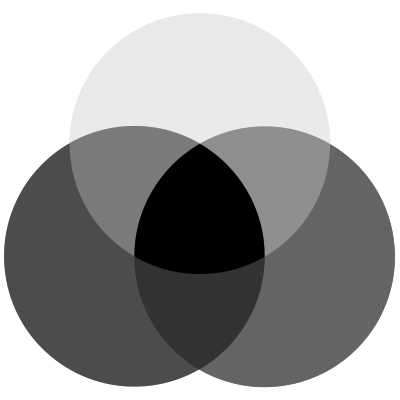
\includegraphics[width=0.28\columnwidth]{venn_gray.png}
\caption{Imagem do arquivo venn\_gray.jpg}
\end{center}
\end{figure}

Com a mesma facilidade é possível abrir uma imagem em níveis de cinza.

\begin{lstlisting}[language=bash]
$> python requisito1.py
(line, column):(178,129); Luminosity (122)
\end{lstlisting}
\subsection*{Aplicação 2}
Com imagens coloridas e em tons de cinza, a \textit{Aplicação 2} colore o ponto clicado de vermelho.
\begin{figure}[h!]
\begin{center}

\includegraphics[width=0.28\columnwidth]{requisito2_color.png}
\caption{Coloração de uma imagem RGB}
\end{center}
\end{figure}
\begin{figure}[h!]
\begin{center}
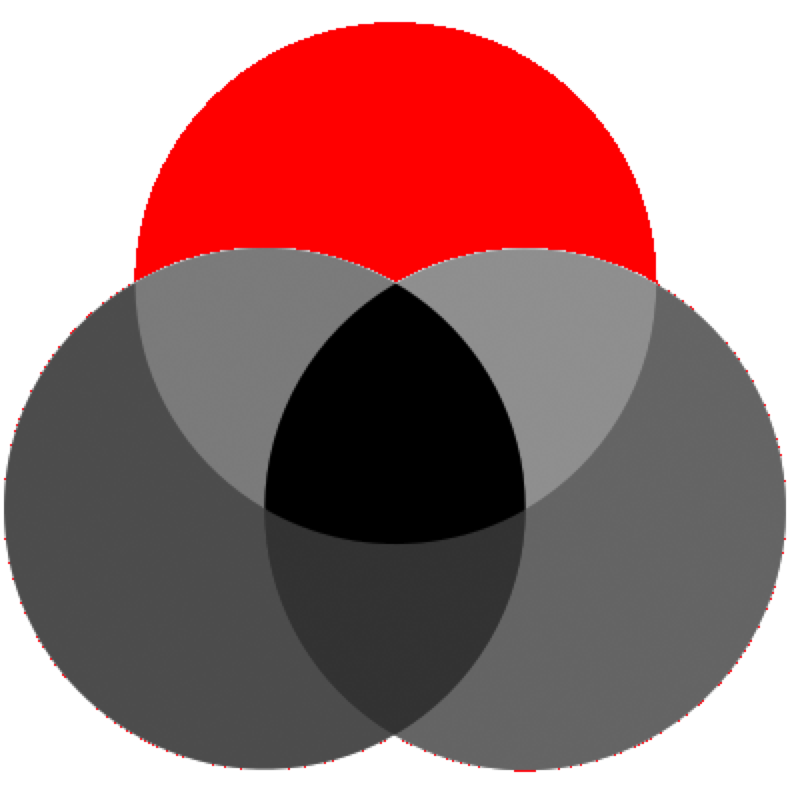
\includegraphics[width=0.28\columnwidth]{requisito2_gray.png}
\caption{Coloração de uma imagem Grayscale}
\end{center}
\end{figure}
\subsection*{Aplicação 3}
O uso de vídeo impõe maior necessidade de eficiência no processamento. Usando um vídeo pequeno (180 x 320, em padrão x.264), a Aplicação 3 funciona sem problemas.

A Tabela I compara a mediana do tempo da coloração usando operação de matrizes em relação a uma abordagem ingênua com \textit{forloop}:

\begin{minipage}{\linewidth}
\centering
\captionof{table}{Processamento da Coloração} \label{tab:title} 
\begin{tabular}{ C{.755in} C{.85in} *4{C{.75in}}}\toprule[1.5pt]
\bf Algoritmo & \bf Mediana ms/frame  \bf \\\midrule
Matrizes        &  3.37 \\
ForLoop        &  1615.26 \\
\bottomrule[1.25pt]
\end {tabular}\par

\end{minipage}

\begin{figure}[h!]
\begin{center}
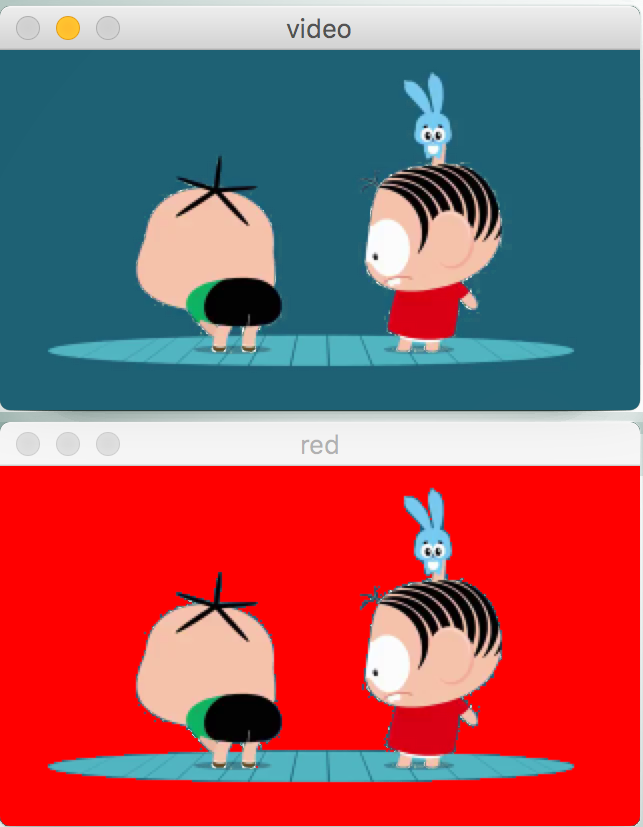
\includegraphics[width=0.66\columnwidth]{toy.png}
\caption{Coloração de vídeo}
\end{center}
\end{figure}


\subsection*{Aplicação 4}
Com OpenCV, usar a imagem \textit{stream} da webcam ao invés de um arquivo de vídeo é trivial.
\begin{figure}[h!]
\begin{center}
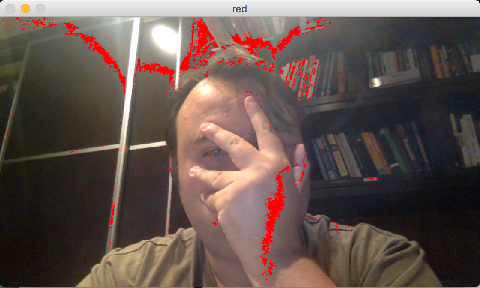
\includegraphics[width=0.66\columnwidth]{cam.png}
\caption{Coloração do \textit{stream} da webcam}
\end{center}
\end{figure}

\section{Discussão e Conclusões}
Os resultados obtidos confirmam a ideia de que OpenCV é uma ferramenta importante para facilitar o acesso a área de Visão Computacional. 
Além disto, conseguimos constatar que o uso de operações de matrizes é muito mais eficiente (cerca de 480X mais rápida) que a abordagem ingênua. 
Ao longo do projeto, identificou-se que outras abordagens para coloração poderiam melhorar ainda mais o resultado: 
\begin{itemize}
\item Poderíamos utilizar uma abordagem multiprocessada e mover o processamento da coloração para uma thread separada da leitura dos frames do vídeo.
\item Poderíamos usar a OpenCV para converter os frames de vídeo para o espaço de cores HSL e checar a similaridade dos pixels nesse outro espaço.
\end{itemize}
Nenhuma dessas ideias, entretanto, faziam parte do escopo do projeto e ficam como sugestão para novas pesquisas.
% \begin{thebibliography}{00}
% \bibitem{b1} G. Eason, B. Noble, and I. N. Sneddon, ``On certain integrals of Lipschitz-Hankel type involving products of Bessel functions,'' Phil. Trans. Roy. Soc. London, vol. A247, pp. 529--551, April 1955.
% \bibitem{b2} J. Clerk Maxwell, A Treatise on Electricity and Magnetism, 3rd ed., vol. 2. Oxford: Clarendon, 1892, pp.68--73.
% \bibitem{b3} I. S. Jacobs and C. P. Bean, ``Fine particles, thin films and exchange anisotropy,'' in Magnetism, vol. III, G. T. Rado and H. Suhl, Eds. New York: Academic, 1963, pp. 271--350.
% \bibitem{b4} K. Elissa, ``Title of paper if known,'' unpublished.
% \bibitem{b5} R. Nicole, ``Title of paper with only first word capitalized,'' J. Name Stand. Abbrev., in press.
% \bibitem{b6} Y. Yorzu, M. Hirano, K. Oka, and Y. Tagawa, ``Electron spectroscopy studies on magneto-optical media and plastic substrate interface,'' IEEE Transl. J. Magn. Japan, vol. 2, pp. 740--741, August 1987 [Digests 9th Annual Conf. Magnetics Japan, p. 301, 1982].
% \bibitem{b7} M. Young, The Technical Writer's Handbook. Mill Valley, CA: University Science, 1989.
% \end{thebibliography}


\selectlanguage{brazilian}
\bibliographystyle{IEEEtran}
\bibliography{references}
\end{document}
